\documentclass[a4paper]{article}

%% Language and font encodings
\usepackage[french]{babel}
\usepackage[utf8]{inputenc}
\usepackage[T1]{fontenc}

\usepackage{float}

\usepackage{algorithm}
\usepackage[noend]{algpseudocode}
\algnewcommand{\algorithmicand}{\textbf{ and }}
\algnewcommand{\algorithmicor}{\textbf{ or }}
\algnewcommand{\OR}{\algorithmicor}
\algnewcommand{\AND}{\algorithmicand}
\algnewcommand\algorithmicforeach{\textbf{for each}}
\algdef{S}[FOR]{ForEach}[1]{\algorithmicforeach\ #1\ \algorithmicdo}


%% Sets page size and margins
\usepackage[a4paper,top=3cm,bottom=2cm,left=3cm,right=3cm,marginparwidth=1.75cm]{geometry}

%% Useful packages
\usepackage{amsmath}
\usepackage{amssymb}
\usepackage{graphicx}
\usepackage[colorinlistoftodos]{todonotes}
\usepackage[colorlinks=true, allcolors=blue]{hyperref}
\usepackage{graphicx}

\usepackage[backend=biber,uniquename=init,giveninits=true,
             %% "et al" pour > deux auteurs, & pour exactement 2
             uniquelist=false,maxcitenames=2,mincitenames=1,maxbibnames=99,
             isbn=false,url=false,doi=false,bibstyle=numeric
]{biblatex}
\addbibresource{references.bib}

\title{Document de travail}
\author{Laura Nguyen}

\begin{document}
\maketitle

\section{Introduction} Dans beaucoup de problèmes de classification, les valeurs
des attributs et de la classe sont ordinaux. De plus, il peut exister une
contrainte de monotonie: la classe d'un objet doit croître/décroître en fonction
de la valeur de tout ou partie de ses attributs.  A savoir, étant donné deux
objets $x, x'$, si $x \leq x'$ alors $f(x) \leq f(x')$. Les variables
dépendantes, $f(x)$ et $f(x')$, sont des fonctions monotones des variables
indépendantes, $x$ et $x'$.
On parle alors de problèmes de classification monotone, ou problèmes de
classification avec contrainte de monotonie. Cette contrainte indique que les
objets ayant de meilleures valeurs d'attributs ne doivent pas être assignés à de
moins bonnes valeurs de classe.\\
L'ajout de cette contrainte de monotonie permet d'introduire des concepts
sémantiques tels la préférence, la priorité, l'importance, qui nécessitent une
relation d'ordre.\\ Il existe de nombreux domaines se prêtant à ce type de
tâches, tels la prédiction du risque de faillite \cite{greco-new-bankruptcy},
l'analyse de la satisfaction des clients \cite{greco-customer}, le diagnostic
médical \cite{marsala-gradual}. 
L'importance de la prise en compte d'une relation graduelle entre les valeurs
d'attributs et la classe a été démontrée \cite{pazzani-acceptance}: les
classifieurs auxquels sont imposés la contrainte de monotonie sont au moins
aussi performants que leurs homologues classiques, et les experts sont plus
enclins à utiliser les règles générées par les modèles monotones.\\
Afin d'extraire des règles à partir de données monotones, on décide d'utiliser
les arbres de décision, dont l'efficacité et l'interprétabilité en
classification a été prouvée \cite{quinlan-induction}.  Cependant, les
algorithmes de construction d'arbres de décision standards (générés par CART
\cite{leo-classification}) ne produisent pas de classifieurs sensibles à la
monotonie, même si la base utilisée est complètement monotone.  En revanche, il
est montré dans \cite{ben-adding} que les classifieurs purement monotones
(\cite{ben-learning}, \cite{ben-monotonicity}, \cite{cao-consistent}) sont, en
terme de taux de bonne classification, statistiquement indiscernables de leurs
homologues non-monotones.  Dans le même article, il est expliqué que ce
phénomène est dû à la sensibilité de ces classifieurs au bruit non-monotone
présent dans les données réelles. \\

Ce stage a pour but d'étudier la construction et l'évaluation d'arbres de
décision prenant en compte une relation graduelle susceptible d'exister entre
les valeurs d'attributs et la classe, tout en étant suffisamment robuste au
bruit non-monotone. On reprend, en particulier, \cite{marsala-rank} pour la
construction d'arbres de décision monotones paramétrés par une mesure de
discrimination d'ordre. Une étude théorique des propriétés des mesures présentées
dans le même article est également effectuée.\\

\section{Etat de l'art} 
Dans cette partie, on étudie et compare les méthodes proposées par Hu et al.
\cite{hu-rank}, Marsala et Petturiti \cite{marsala-rank}, Qian et al.
\cite{qian-fusing} et Pei et Hu \cite{pei-partially}.

\subsection{Notations}
On considère un ensemble $\Omega = \{\omega_1,...,\omega_n\}$ d'éléments définis
par un ensemble d'attributs $A = \{a_1,...,a_m\}$, où pour tout $j=1,...,m, a_j$
est une fonction de $\Omega$ vers $X_j = \{x_{j_1},...,x_{t_j}\}$. On note aussi
$\lambda: \Omega \rightarrow C$ la fonction d'étiquetage, où $C =
\{c_1,...,c_k\}$ est un ensemble de classes totalement ordonné.

Pour $\omega_i \in \Omega$, l'ensemble dominant de $\omega_i$ généré par $a_j$
est défini de la façon suivante :

$$[\omega_i]^{\leq}_{a_j} = \{w_h \in \Omega : a_j(\omega_i) \leq a_j(\omega_h)\}$$

De même, l'ensemble dominant de $\omega_i$ généré par $\lambda$ s'écrit :

$$[\omega_i]^{\leq}_{\lambda} = \{w_h \in \Omega : \lambda(\omega_i) \leq
\lambda(\omega_h)\}$$ \\

Les notions de \textit{dominance rough sets} sont également utilisées. On
cherche à approximer l'ensemble $c^{\geq}_q$, ie l'ensemble des éléments de
$\Omega$ dont la valeur de classe est inférieure à $c_q$.

\noindent Soit $B \subseteq A$ et $c_q$ une valeur de classe. Les approximations
inférieure et supérieure de $c^{\geq}_q$ sont définis de la façon suivante:

$$ \underline{R^{\geq}_B}(c^{\geq}_q) = \{\omega \in \Omega :
[\omega]^{\geq}_B \subseteq c^{\geq}_q\}$$

$$ \overline{R^{\geq}_B}(c^{\geq}_q) = \{\omega \in \Omega :
[\omega]^{\leq}_B \cap c^{\geq}_q \neq \varnothing\}$$


\subsection{Arbre de décision basé sur l'entropie d'ordre}
Il est montré dans \cite{ben-adding} que les classifieurs purement monotones ne
procurent pas de meilleurs résultats que leurs homologues classiques lorsque les
données contiennent un taux élevé de bruit non-monotone. 

Afin de résoudre ce problème, les auteurs de \cite{hu-rank} proposent un algorithme robuste pour la
classification monotone.

Pour cela, ils définissent une mesure de degré de monotonie entre deux
attributs, qu'ils nomment information mutuelle d'ordre, ou
\textit{rank mutual information} (RMI): \\
$$ RMI^{\leq}(a_j, a_{j'}) = -\frac{1}{n} \sum_{i=1}^{n} \log
\frac{|[\omega_i]^{\leq}_{a_j}]| \times |[\omega_i]^{\leq}_{a_{j'}}]|}{n \times
|[\omega_i]^{\leq}_{a_j}]\cap [\omega_i]^{\leq}_{a_{j'}}]|}$$

RMI, sensible à la monotonie et robuste face aux données bruitées, est utilisé
comme mesure de sélection d'attribut dans leur algorithme de construction
d'arbres de décision monotones, REMT (\textit{Rank Entropy Based Decision
Tree}).

Dans cet article, on considère seulement les arbres binaires dans lesquels
est affecté à chaque noeud un seul attribut. Concernant les données, les
attributs doivent être numériques et la classe, ordinale.


\noindent A chaque étape de l'induction :
\begin{itemize}
    \item si $|\Omega_{\alpha}| = 1$ ou tous les éléments
de $\Omega_{\alpha}$ partagent la même classe, une feuille est créée. 
    \item Sinon, pour chaque attribut $a_j$, pour chaque valeur d'attribut $x_{j_s}$, l'ensemble
des éléments est divisé en deux sous-ensembles à partir desquels on calcule
$RMI_{x_{j_s}} = RMI(a^{x_{j_s}}_j, \lambda)$. On récupère, pour chaque $a_j$,
le seuil de coupure $x^*_j$ maximisant l'information mutuelle d'ordre :
$x^*_{j_s} = arg\,max RMI_{x_{j_s}}.$ L'attribut $a^*$ utilisé pour le
partitionnement est celui dont le seuil $x^*$ maximise
$RMI(a^{x_{j_s}}_j,\lambda)$, pour $j=1,...,m, s=1,...t_j-1.$ 
    \item Si $RMI(a^*,
\lambda) < \epsilon$, une feuille est créée. 
    \item Sinon, un noeud est construit et la
procédure est répétée sur les sous-ensembles induits par $a^*$ et $x^*$. \\
\end{itemize}

Concernant le critère d'étiquetage, si tous les exemples de la feuille possèdent
la même classe, on lui assigne cette dernière. Sinon, si les exemples
proviennent de classes différentes, on assigne la classe médiane. Dans le cas où
deux classes possèdent le même nombre d'exemples et la feuille courante provient
de la branche gauche de son noeud parent, on lui assigne la pire classe. Sinon,
on lui affecte la meilleure.  \\

L'approche de construction gloutonne du classifieur ne permet pas d'obtenir un
arbre globalement monotone, même si les données utilisées sont monotones. En
revanche, cette méthode garantit une monotonie plus faible : il est montré que
si la base de données utilisée lors de la construction de l'arbre est
monotone-consistente, alors les règles générées par REMT sont monotones. \\

Afin d'évaluer la performance de leur algorithme, Hu et al. utilisent l'erreur absolue moyenne, ou
\textit{Mean Absolute Error} (MAE) :
$$ MAE = \frac{1}{n} \sum_{i=1}^{n}|f(\omega_i) - \lambda(\omega_i)| $$
où $f(\omega_i)$ est la classe prédite par REMT. \\

L'algorithme est testé sur des bases de données artificielles et réelles. 

\noindent Les bases de données artificielles générées sont monotones. Elles contiennent
1000 exemples à deux attributs, et un nombre de classes variant de 2 à 30. 

\noindent REMT est ici comparé à CART, Rank Tree \cite{xia-ranking}, OLM
\cite{ben-learning} et OSDL \cite{cao-supervised}. Les expériences montrent que
REMT produit le moins d'erreurs parmi ces algorithmes, hormis dans le cas à deux
classes.  Les auteurs soulignent aussi que REMT est le plus précis des quatre
algorithmes, peu importe le nombre d'éléments utilisés lors de la construction
de l'arbre.


Sur des bases de données réelles, Hu et al. comparent leur modèle à CART et Rank
Tree \cite{xia-ranking}. Les expériences menées montrent que REMT donne de
meilleurs résultats en termes de MAE sur 10 bases sur les 12 collectées. De
plus, les auteurs montrent également que plus la taille de la base
d'apprentissage diminue, plus l'écart de performance se creuse entre REMT et les
autres modèles. 
\noindent Enfin, dans le but de comparer les performances des algorithmes
lorsque les données sont monotones, les mêmes bases sont modifiées à l'aide d'un
algorithme de monotonization . Les résultats des expérimentations montrent que
REMT est plus performant que les autres modèles. De plus, les valeurs de
MAE produites par tous les modèles diminuent lorsque les données sont
monotisées.

\subsection{Arbre de décision paramétré par une mesure de discrimination
d'ordre} 
Dans \cite{marsala-rank}, Marsala et Petturiti étudient l'influence de
la mesure de discrimination utilisée lors de la construction du classifieur, en
termes de taux de bonne prédiction et de monotonie. 

Comme les mesures étudiées dans l'article partagent toutes la même structure
fonctionnelle, les auteurs définissent un modèle de construction hiérarchique
permettant d'isoler les propriétés d'une mesure de discrimination d'ordre et
d'en créer de nouvelles. \\
Soit $H^*$ une mesure de discrimination d'ordre. Le pouvoir de discrimination de
l'attribut $a_j$ envers $\lambda$ selon $H^*$ peut donc s'écrire de la façon suivante :
$$ H^*(\lambda | a_j) = h^*(g^*(f^*(\omega_1)),...,g^*(f^*(\omega_n)))$$

Marsala et Petturiti proposent un algorithme de construction d'arbre de décision
nommé RDMT (\textit{Rank Discrimination Measure Tree}) essentiellement basé sur
REMT mais qui utilise, à la place de RMI, une mesure de discrimination passée en paramètre.

\noindent Comme précédemment, seuls les arbres binaires à un attribut par noeud
sont considérés. Ce classifieur gère à la fois les attributs numériques et ordinaux, mais la classe
doit être ordinale. \\

Notons H la mesure de discrimination utilisée, $\epsilon$ le seuil minimal pour
H, $\Omega_{\alpha}$ l'ensemble des exemples considérés à l'étape courante de
construction, $\alpha$ la taille minimale pour $\Omega_{\alpha}$, $\delta$ la
profondeur courante de la branche, et $\Delta$ la profondeur maximale que peut
avoir une branche de l'arbre. \\

\noindent A chaque étape de l'induction :
\begin{itemize}
    \item si $|\Omega_{\alpha}| < \alpha$ ou tous les éléments
de $\Omega_{\alpha}$ partagent la même classe ou $\delta > \Delta$, une feuille est créée. 
    \item Sinon, pour chaque attribut $a_j$, pour chaque valeur d'attribut $x_{j_s}$, l'ensemble
des éléments est divisé en deux sous-ensembles à partir desquels on calcule
        $H(\lambda|a^{x_{j_s}}_j)$. On récupère, pour chaque $a_j$,
le seuil de coupure $x^*_j$ minimisant la valeur de H:
$x^*_{j} = arg\,min H(\lambda|a^{x_{j_s}}_j)$. L'attribut $a^*$ utilisé pour le
partitionnement est celui dont le seuil $x^*$ minimise
$H(\lambda|a^{x_{j_s}}_j)$, pour $j=1,...,m, s=1,...t_j-1.$ 
    \item Si $H(\lambda|a^*) < \epsilon$, une feuille est créée. 
    \item Sinon, un noeud est construit et la
procédure est répétée sur les sous-ensembles induits par $a^*$ et $x^*$. \\
\end{itemize}

\noindent Comme REMT, RDMT ne garantit pas un classifieur globalement monotone, mais
un arbre générant des règles monotones.  \\

Les auteurs évaluent les modèles construits selon trois critères: le taux de bonne
classification (mesuré par le pourcentage d'exemples correctement étiquetés, le
test du K, et MAE), la monotonie et la taille des arbres (en termes de nombre de
feuilles). 
\noindent La monotonie d'un arbre est évaluée par deux mesures :
\begin{itemize}
    \item L'index I de non-monotonie d'un arbre $\mathcal{T}$:  
        $$ I(\mathcal{T}) = \frac{\sum_{u=1}^q \sum_{v=1}^{q} m_{u,v}}{q^2 - q}$$
        où q est le nombre de feuilles de $\Gamma$ et $m_{u,v}$ vaut 1 si les
        feuilles $l_u, l_v$ ne sont pas monotones, 0 sinon.
    \item L'index NMI1 des exemples dans chaque base de test $\mathcal{D}$:
        $$ NMI1(\mathcal{D}) = \frac{\sum_{i=1}^n \sum_{h=1}^{n} NMP(\omega_i,
        \omega_h)}{n^2 - n}$$
        où $NMP(\omega_i, \omega_h)$ vaut 1 si la paire $\omega_i, \omega_h$
        n'est pas monotone, 0 sinon. \\
\end{itemize}

Les expérimentations menées dans l'article visent à comparer les arbres obtenus
par différentes mesures ($H^*_S, H_S, H^*_G, H_G, H^*_P, H^{10}_{MID}, H_{ICT}$).

11 bases artificielles sont générées, dont le taux de NMI augmente de 0 à 10\%
avec un pas de 1\%. Chaque base contient 500 exemples à 5 attributs et 5
classes. \\
\noindent Les tests menés sur ces bases montrent qu'il n'existe aucune
différence significative entre les mesures en ce qui concerne les indices de
taux de bonne classification. De plus, les mesures de discrimination d'ordre
produisent des arbres plus monotones, en particulier lorsque le taux de bruit
non-monotone de la base augmente. Enfin, il est également montré que ces mesures
de discrimination produisent des arbres contenant plus de feuilles que les
mesures classiques.

15 bases de données réelles sont séléctionnées pour évaluer les mesures sur des
cas d'applications concrets. Comme précédemment, il n'y a pas de différence
de taux de bonne classification significative entre les mesures. Cependant,
$H^*_S, H^*_G,$ et $H^*_P$ génèrent des arbres plus monotones et comportant
davantage de feuilles. \\

Les arbres produits par des mesures de discrimination d'ordre ne sont pas
destinés à être directement utilisés pour la classification monotone. En
revanche, étant donné leur degré de monotonie plus élevé, il est avantageux de
les passer en entrée d'algorithmes de post-traitement afin renforcer la
monotonie globale.

\subsection{Fusion d'arbres de décision monotones} 
Afin d'améliorer la capacité de généralisation du modèle de classification, Qian
et al. dans \cite{qian-fusing} proposent une méthode d'ensemble par fusion
d'arbres de décision monotones, notée FREMT (\textit{Fusing rank entropy based
monotonic decision trees}).

Les auteurs couplent une méthode de réduction d'attributs préservant l'ordre
avec REMT, utilisé pour générer les classifieurs de base.

Pour réduire l'ensemble des attributs, ils se basent sur les \textit{dominant
rough sets} et mettent à jour leur définition. Ils introduisent un paramètre
$\beta$ qui permet de paramétrer la sensibilité du \textit{rough set} au bruit
non-monotone. L'ensemble à approximer est : 
$$c^{\geq}_q = \bigcup_{u \leq q} C_u$$
où $C_u \in \Omega / \lambda = \{C_1, C_2,...,C_r\}$ tel que, pour tout $q, u \leq r$, si $q
\geq u$ alors les éléments de $C_q$ sont préférés à ceux de $C_u$.

\noindent Soit $B \subseteq A$ et $c_q$ une valeur de classe. Les approximations
inférieure et supérieure de $c^{\geq}_q$ sont définis de la façon suivante:

$$ \underline{R^{\geq}_B}(c^{\geq}_q) = \{\omega \in \Omega :
\frac{|[\omega]^{\geq}_B \cap c^{\geq}_q|}{|[\omega]^{\geq}_B|} \geq 1 -
\beta\}$$

$$ \overline{R^{\geq}_B}(c^{\geq}_q) = \{\omega \in \Omega :
\frac{|[\omega]^{\geq}_B \cap c^{\geq}_q|}{|[\omega]^{\geq}_B|} \geq \beta\}$$

\noindent où $0 \leq \beta \leq 0.5$

\noindent La frontière ascendante de $c_q$ liée à l'ensemble d'attributs B s'écrit :

$$ BND^{\beta}_B(c^{\geq}_q) = \overline{R^{\geq}_B}(c^{\geq}_q) - \underline{R^{\geq}_B}(c^{\geq}_q)$$

\noindent La dépendance monotone de $\lambda$ selon B est donc exprimée de la façon
suivante :

$$ \gamma^{\beta}_B(\lambda) = \frac{|\Omega - \bigcup_{q=1}^k
BND^{\beta}_B(c^{\geq}_q)|}{|\Omega|}$$

\noindent A partir de cette définition, il est possible d'établir un coefficient de
pertinence d'un attribut a dans B, relativement à $\lambda$. La pertinence
interne de a dans B relativement à $\lambda$ est définie de la manière suivante
:

$$ Sig^{\beta}_{inner}(a, B, \lambda) = \gamma^{\beta}_B(\lambda) -
\gamma^{\beta}_{B-\{a\}}(\lambda)$$

\noindent De la même façon, $\forall a \in A-B$, la pertinence externe de a selon B
correspond à :

$$ Sig^{\beta}_{outer}(a, B, \lambda) = \gamma^{\beta}_{B \cup \{a\}}(\lambda) -
\gamma^{\beta}_B(\lambda)$$ \\

À l'aide de ces mesures de pertinence d'attributs, Qian et al. proposent un
algorithme de réduction d'attributs, paramétré par $\beta$, qui, étant donné
$\Omega$,~$A$ et $\lambda$, génère une réduction (\textit{reduct}) d'attributs
monotones. Le principe est le suivant :

\begin{itemize}
    \item On récupère dans~$B$ les attributs noyaux de~$B$ en utilisant
        $Sig^{\beta}_{inner}$.
    \item Pour tout attribut $a_j \in A-B$, on calcule $Sig^{\beta}_{outer}(a_j,
        B, \lambda)$. 
    \begin{itemize}
        \item Si la valeur calculée est supérieure ou égale à toutes celles obtenues
            précédemment, alors on rajoute $a_j$ dans~$B$.
        \item on réitère le processus jusqu'à ce que, pour tout $a_i \in A-B$,
            $Sig^{\beta}_{outer}(a_i, B, \lambda) = 0$ (i.e. rajouter $a_i$
            à~$B$ ne modifie pas $\gamma^{\beta}_{B}(\lambda)$).
    \end{itemize}
\end{itemize}

\noindent Comme la taille de l'ensemble des attributs monotones sélectionnés par cette
méthode est bien moindre que celle de l'ensemble original, l'arbre de décision
induit par ces attributs sera moins profond et contiendra moins de noeuds, ce
qui implique une meilleure aptitude à généraliser. Chaque arbre produit par cet
algorithme sert de classifieur de base pour la méthode d'ensembles.

Afin d'obtenir un classifieur final performant, il est nécessaire de produire
des arbres les plus diversifiés possibles. Plusieurs sous-ensembles d'attributs
sont donc sélectionnés, et chacun de ces sous-ensembles est une réduction d'attributs
qui préserve la monotonie des données. 

\noindent Les auteurs définissent donc une méthode de recherche de multiples réductions
d'attributs monotones, paramétrée par $\beta$. Étant donné $\Omega$,~$A$ et
$\lambda$, elle consiste à :
\begin{itemize}
    \item Trouver les attributs noyaux de A en utilisant $Sig^{\beta}_{inner}$.
    \item Trier par ordre croissant les attributs restants $a_j \in B$ en fonction de
        $\gamma^{\beta}_{B} + \frac{|\Omega / \{a_j\}|}{|\Omega|}$.
    \item Stocker dans $P^*$ les deux sous-ensembles précédents.
    \item À partir de $P^*$, trouver une réduction
d'attributs $RED_0$ avec l'algorithme de réduction d'attributs donné plus haut.
    \item Pour chacun des attributs $a_j$ se trouvant dans $RED_0$ mais n'étant
        pas des attributs noyaux,
    \begin{itemize}
        \item Enlever $a_j$ de $P^*$.
        \item Calculer une réduction $RED_j$ à partir de $P^*$ grâce à
            l'algorithme précédent.
        \item Si $RED_j$ n'a pas déjà été trouvée précédemment, rajouter $RED_j$
            à l'ensemble des réductions obtenues.
        \item Remettre $a_j$ dans $P^*$.
    \end{itemize}
\end{itemize}

\noindent Cette méthode permet de générer un ensemble de réductions d'attributs monotones
aussi diversifié que possible. Ces sous-ensembles d'attributs servent de base pour construire des arbres de
décision complémentaires, générés par REMT. 

Soit $F = \{T_1,T_2,...,T_N\}$ une forêt d'arbres de décision générés par $RED =
\{RED_1,RED_2,...,RED_N\}$. Étant donnés $\Omega$, $A$, $\lambda$,
$\beta = \{\beta_1,\beta_2,\}$, et $\omega$ un objet dont la classe est à
déterminer, l'algorithme final de fusion d'arbres de décision
monotones, \textit{Fusing rank entropy based monotonic decision trees (FREMT)},
est le suivant :
\begin{itemize}
    \item Pour $i=1,...,M$, trouver $RED_i = \{RED_0,RED_1,...,RED_{N_i}\}$ avec
        l'algorithme précédent
    \item Stocker dans $RED$ l'union de tous les ensembles de réductions $RED_i$ générés
    \item Pour chaque $RED_j \in RED$, générer un arbre $T_j$ avec REMT.
    \item Construire F la forêt d'arbres $\{T_1,T_2,...,T_N\}$.
    \item Déterminer la classe de $\omega$ avec F selon le principe de fusion
        basé sur la probabilité maximale (\textit{Fusing principle based on
        maximal probability}). \\
\end{itemize}


Qian et al. évaluent la performance de leur modèle selon le taux de bonne
classification (mesuré par le pourcentage d'instances correctement classifiées)
et l'erreur absolue moyenne. 

Les tests sont menés uniquement sur des bases réelles.

\noindent Sur les 10 bases récupérées, 9 nécessitent un pré-traitement afin
d'être adaptés à l'algorithme de fusion d'arbres (en transformant les problèmes
de monotonie descendantes en problèmes de monotonie ascendantes). De plus, afin
de comparer les performances des modèles lorsque les données sont monotones, les
classes des données sont modifiées à l'aide d'un algorithme de monotonization.

\noindent Les auteurs observent d'abord les performances des arbres constituant
la forêt (construits à partir des réductions d'attributs des données d'origine)
puis la performance du modèle final. Ils comparent leurs résultats à ceux
obtenus par REMT.

\noindent D'après les expériences menées, on observe que les arbres de décision
générés par les réductions d'attributs offrent de meilleurs résultats en termes
de taux de bonne classification et d'erreur absolue moyenne dans la plupart des
cas. De plus, les valeurs générées sont différentes les unes des autres, ce qui
satisfait la contrainte de diversité nécessaire au modèle d'ensembles.
Enfin, le classifieur produit par FREMT s'avère être meilleur que
celui généré par REMT sur toutes les bases considérées, en termes de taux de
bonne classification et d'erreur absolue moyenne. FREMT permet aussi d'améliorer
la capacité de généralisation de REMT sur ces tâches de classification.


\subsection{Arbres de décision partitiellement monotones} 

Dans cette partie, on distingue deux types d'attributs : ceux  dont les valeurs
sont linéairement ordonnées selon les valeurs de la classe, qu'on appelle
critères, et ceux n'ayant pas de relation monotone avec la classe. La plupart
des tâches de classification monotone comprennent ces deux sortes d'attributs.
Cependant, les algorithmes étudiés précédemment font l'hypothèse que tous les
attributs sont monotones par rapport à la classe. On ne peut néanmoins pas
conserver uniquement les critères car les autres attributs permettent
d'améliorer la performance du classifieur. Dans \cite{pei-partitially},
Pei et Hu proposent donc un algorithme de construction d'arbres partiellement
monotones permettant de gérer les deux types d'attributs à la fois. 


Pour cela, ils proposent une mesure d'inconsistence d'ordre, \textit{rank
inconsistency rate} (RIR), qui permet de distinguer les attributs ordinaires des
critères et de déterminer les sens des relations graduelles entre les critères
et la classe.

\section{Etude théorique des propriétés des mesures de discrimination d'ordre}
Marsala et Petturiti définissent dans \cite{marsala-rank} un modèle de
construction hiérarchique de mesures de discrimination d'ordre. Ce modèle a pour
but d'isoler les propriétés qu'une fonction doit avoir pour être une telle
mesure. Il sert aussi de base pour en créer de nouvelles. \\

Soit $H^*$ une mesure de discrimination d'ordre. On rappelle que le pouvoir de
discrimination de l'attribut $a_j$ envers la classe $\lambda$ peut se décomposer
de la façon suivante :

$$ H^*(\lambda|a_j) = h^*(g^*(f^*(\omega_1),...,g^*(f^*(\omega_n))))$$

où $f^*$ est une mesure de la monotonie locale de l'objet, $g^*$ une mesure
de non-monotonie de l'objet, et $h^*$ une agrégation des mesures $g^*$.

Pour que $H^*$ soit une mesure de discrimination d'ordre, chaque couche doit
satisfaire certaines conditions.

Soient $\omega_i \in \Omega$ et $f^*, g^*, h^*$ les trois couches de $H^*$. Les propriétés suivantes sont
démontrées en annexe :


\section{Implémentation et expérimentation de l'algorithme de construction
d'arbres monotones} 
On implémente une librarie de fonctions permettant la
construction ainsi que l'étude expérimentale d'arbres de décision.  On se base
essentiellement sur RDMT(H), donné dans \cite{marsala-rank}, pour construire des
arbres de décision monotones, que l'on évalue sur des données artificielles et
réelles. Le code est implémenté en Python 3.6 et les librairies numpy,
matplotlib et scikit-learn sont utilisées.

%\subsection{Aspects calculatoires}
%Dans cette partie, on cherche à évaluer les complexités temporelle et spatiale
%du critère de partitionnement en fonction de la mesure de discrimination
%utilisée. Les mesures de discrimination d'ordre proposées sont basées sur les
%ensembles dominants, et, celles ne tenant pas compte de la monotonie des données,
%sur les classes d'équivalence. Le stockage des ces structures joue donc un rôle
%important dans la complexité du critère de partitionnement. \\
%
%Étant donnés $\Omega = \{\omega_i, ... , \omega_n\}, \mathcal{A} = \{a_1, ...,
%a_m\}, \lambda$, et $j \in \{1, ..., m\}$ fixé, on stocke l'ensemble dominant
%généré par l'attribut $a_j$ (respectivement la fonction d'étiquetage $\lambda$)
%dans une matrice notée~$A$ (respectivement~$D$) de taille $n \times n$. Pour tout $i,
%h \in \{1,...,n\}$,
%\begin{itemize} 
%    \item $A_{ih} = 1$ si et seulement si $a_j(\omega_i) \leq
%a_j(\omega_h)$ ;
%    \item $D_{ih}= 1$ si et seulement si~$\lambda(\omega_i) \leq \lambda(\omega_h)$.
%\end{itemize}
%
%A (respectivement D) est donc rempli en itérant sur chaque $\omega_i \in \Omega$
%et en assignant à chaque ligne $A_i$ (respectivement $D_i$) l'ensemble
%$\{\omega_h : a_j(\omega_i) \leq a_j(\omega_h)\}$ (respectivement $\{\omega_h :
%\lambda(\omega_i) \leq \lambda(\omega_h)\}$). Récupérer ce dernier se fait en
%temps $\mathcal{O}(n)$. On construit donc A et D en temps $\mathcal{O}(n^2)$.
%Comme les valeurs sont stockées dans une matrice de taille $n \times n$, la
%complexité spatiale est aussi en $\mathcal{O}{n^2}$.
%
%En ce qui concerne les classes d'équivalence, pour tout $i, h \in \{1,...,n\}$,
%\begin{itemize}
%    \item $A_{ih} = 1$ si et seulement si $a_j(\omega_i) = a_j(\omega_h)$
%    \item $D_{ih} = 1$ si et seulement si $\lambda(\omega_i) = \lambda(\omega_h)$. 
%\end{itemize}
%La procédure de construction est la même que celle donnée
%précédemment, en remplaçant l'inégalité par l'égalité. On obtient les mêmes
%complexités temporelle et spatiale. Comme les algorithmes maniant les ensembles
%dominants et ceux utilisant les classes d'équivalence partagent les mêmes
%complexités, on étudiera uniquement les fonctions faisant intervenir les
%ensembles dominants. 
%
%Pour $a_j$ donné,~$A$ et~$D$ ne sont calculés qu'une seule fois. \\
%
%Pour calculer $dsr(\omega_i)$, on récupère $[\omega_i]^{\leq}_{a_j}$ et
%$[\omega_i]^{\leq}_{\lambda}$ en temps $\mathcal{O}(n)$. Le calcul de
%$[\omega_i]_{a_j} \cap [\omega_i]_{\lambda}$ étant aussi en $\mathcal{O}(n)$,
%calculer $dsr(\omega_i)$ se fait en temps $\mathcal{O}(n)$. L'espace occupé est
%en $\mathcal{O}(n)$.  En revanche, le calcul de $maxdsr(\omega_i), mindsr(\omega_i)$ et
%$avgdsr(\omega_i)$ nécessite d'itérer sur chaque $\omega_h \in
%[\omega_i]_{a_j}$. Les complexités temporelle et spatiale de ces fonctions sont
%donc en $\mathcal{O}(n^2).$
%
%Toutes les fonctions $g^*$ implémentées sont en $\mathcal{O}(1)$.
%

\subsection{Mesures de discrimination d'ordre} 
On implémente le modèle de
construction hiérarchique proposé par Marsala et Petturiti. On rappelle que le
pouvoir de discrimination de l'attribut $a_j$ envers la classe $\lambda$ selon
une mesure de discrimination $H^*$ peut s'écrire de la façon suivante :

$$ H^*(\lambda | a_j) = h^*(g^*(f^*(\omega_1)),...,g^*(f^*(\omega_n)))$$

\noindent Toutes les fonctions $f^*$, $g^*$, $h^*$ présentées dans l'article
sont codées.  Pour chaque fonction $f^*$, on distingue le cas où la mesure
construite détecte la monotonie (i.e. elle considère les ensembles dominants) du
cas contraire (i.e.  elle considère les classes d'équivalences). \\

Les ensembles dominants et classes d'équivalence servant de base pour le calcul
de $f^*(\omega_i)$, pour tout $\omega_i \in \Omega$, le stockage de ces
structures joue un rôle important dans la complexité du critère de
partitionnement.

Étant donnés $\Omega = \{\omega_i, ... , \omega_n\}, \mathcal{A} = \{a_1, ...,
a_m\}, \lambda$, et $j \in \{1, ..., m\}$ fixé, on stocke les ensembles
dominants générés par l'attribut $a_j$ (respectivement la fonction d'étiquetage $\lambda$) dans une matrice notée~$A$ (respectivement~$D$) de taille $n \times n$. Pour tout $i,
h \in \{1,...,n\}$,
\begin{itemize} 
    \item $A_{ih} = 1$ si et seulement si $a_j(\omega_i) \leq
a_j(\omega_h)$ ;
    \item $D_{ih}= 1$ si et seulement si~$\lambda(\omega_i) \leq \lambda(\omega_h)$.
\end{itemize}
A (respectivement D) est donc rempli en itérant sur chaque $\omega_i \in \Omega$
et en assignant à chaque ligne $A_i$ (respectivement $D_i$) l'ensemble
$\{\omega_h : a_j(\omega_i) \leq a_j(\omega_h)\}$ (respectivement $\{\omega_h :
\lambda(\omega_i) \leq \lambda(\omega_h)\}$). Récupérer ce dernier se fait en
temps $\mathcal{O}(n)$. On construit donc A et D en temps $\mathcal{O}(n^2)$.
Comme les valeurs sont stockées dans une matrice de taille $n \times n$, la
complexité spatiale est aussi en $\mathcal{O}{n^2}$.

En ce qui concerne les classes d'équivalence, pour tout $i, h \in \{1,...,n\}$,
\begin{itemize}
    \item $A_{ih} = 1$ si et seulement si $a_j(\omega_i) = a_j(\omega_h)$
    \item $D_{ih} = 1$ si et seulement si $\lambda(\omega_i) = \lambda(\omega_h)$. 
\end{itemize}
La procédure de construction est la même que celle donnée
précédemment, en remplaçant l'inégalité par l'égalité. On obtient les mêmes
complexités temporelle et spatiale. Comme les algorithmes maniant les ensembles
dominants et ceux utilisant les classes d'équivalence partagent les mêmes
complexités, on étudiera uniquement les fonctions faisant intervenir les
ensembles dominants. 

Pour $a_j$ et $\lambda$ fixés, ~$A$ et~$D$ ne sont calculés qu'une seule fois car
$[\omega_i]^{\leq}_{a_j}$ et $[\omega_i]^{\leq}_{\lambda}$ restent constants,
pour tout $\omega_i \in \Omega$. \\

On s'intéresse maintenant au calcul de $f^*(\omega_i)$, qu'on appelera également
*-$dsr(\omega_i)$.
Afin de calculer $dsr(\omega_i)$, on récupère $[\omega_i]^{\leq}_{a_j}$ et
$[\omega_i]^{\leq}_{\lambda}$ à l'aide de~$A$ et~$D$ en temps $\mathcal{O}(n)$. Le calcul de
$[\omega_i]_{a_j} \cap [\omega_i]_{\lambda}$ se faisant aussi en $\mathcal{O}(n)$,
calculer $dsr(\omega_i)$ se fait en temps $\mathcal{O}(n)$. L'espace occupé est
en $\mathcal{O}(n)$.
En revanche, le calcul de $maxdsr(\omega_i), mindsr(\omega_i)$ et
$avgdsr(\omega_i)$ nécessite d'itérer sur chaque $\omega_h \in
[\omega_i]_{a_j}$. Les complexités temporelle et spatiale de ces fonctions sont
donc en $\mathcal{O}(n^2).$ \\

Afin d'observer le comportement des *-dsr sur un attribut monotone, on génère
une base de 100 points à deux classes, deux dimensions dont une seule est
monotone par rapport à la classe.  Ici, la valeur de l'attribut monotone et
celle de la classe croissent en fonction de l'indice de l'élément. On duplique
et bruite la même base de sorte à obtenir des bases bruitées à 0\%, 25\%, 50\%,
75\%.  Les courbes \ref{img:dsr0}, \ref{img:dsr25}, \ref{img:dsr50}, et
\ref{img:dsr75} tracent la valeur de $dsr(\omega_i)$ en fonction de i pour
chaque base. \\

\begin{figure}[H]
	\center 
	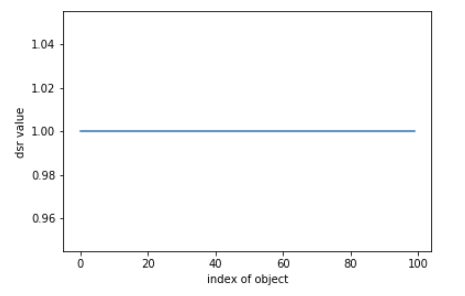
\includegraphics[width=0.6\textwidth]{images/dsr_0.png}
    \caption{Valeur de dsr en fonction de l'indice de l'objet pour une base
    non-bruitée}
    \label{img:dsr0}
\end{figure}

\begin{figure}[H]
	\center 
	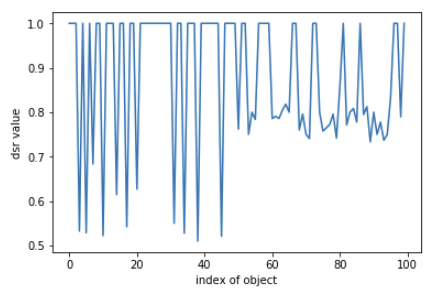
\includegraphics[width=0.6\textwidth]{images/dsr_25.png}
    \caption{Valeur de dsr en fonction de l'indice de l'objet pour une base
    bruitée à 25\%}
    \label{img:dsr25}
\end{figure}

\begin{figure}[H]
	\center 
	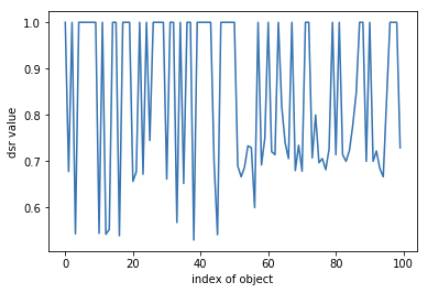
\includegraphics[width=0.6\textwidth]{images/dsr_50.png}
    \caption{Valeur de dsr en fonction de l'indice de l'objet pour une base
    bruitée à 50\%}
    \label{img:dsr50}
\end{figure}

\begin{figure}[H]
	\center 
	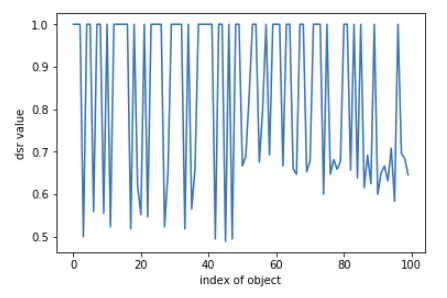
\includegraphics[width=0.6\textwidth]{images/dsr_75.png}
    \caption{Valeur de dsr en fonction de l'indice de l'objet pour une base
    bruitée à 75\%}
    \label{img:dsr75}
\end{figure}

%\begin{figure}[H]
%	\center 
%	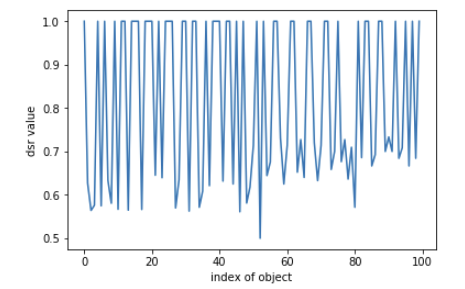
\includegraphics[width=0.6\textwidth]{images/dsr_90.png}
%    \caption{Valeur de dsr en fonction de l'indice de l'objet pour une base
%    bruitée à 90\%}
%    \label{img:dsr90}
%\end{figure}

Dans la base non bruitée, dsr($\omega_i$) = 1 pour chaque $\omega_i \in \Omega$.
En effet, on a $a_j(\omega_i) \leq a_j(\omega_h) \Rightarrow \lambda(\omega_i)
\leq \lambda(\omega_h)$ si et seulement si $\{\omega_h \in \Omega :
\lambda(\omega_i) \leq \lambda(\omega_h) \land a_j(\omega_i) \leq
a_j(\omega_h)\} = \{\omega_h \in \Omega : a_j(\omega_i) \leq a_j(\omega_h)\}$ si
et seulement si $\frac{| [\omega_i]^{\leq}_{\lambda} \cap
[\omega_i]^{\leq}_{a_j}|}{| [\omega_i]^{\leq}_{a_j} |} = 1 $.

\noindent En revanche, plus le taux de bruit dans la base augmente, plus on observe de
"pics". En effet, on observe davantage de $\omega_i$ tels que $ \{\omega_h \in
\Omega : a_j(\omega_i) \leq a_j(\omega_h)\} $ est modifié, et donc  $|
\{\omega_h \in \Omega : \lambda(\omega_i) \leq \lambda(\omega_h) \land
a_j(\omega_i) \leq a_j(\omega_h)\} | \leq | \{\omega_h \in \Omega :
a_j(\omega_i) \leq a_j(\omega_h)\} |$.

\noindent Les courbes des autres *-dsr sont données en annexe.\\

Toutes les fonctions $g^*$ présentées dans l'article ont des complexités
temporelle et spatiale en $\mathcal{O}(1)$. En revanche, comme les fonctions
$h^*$ agrègent les couches $g^*$ correspondant à chaque élément de $\Omega$,
elles sont toutes en $\mathcal{O}(n)$.   

Le calcul de $H^*(\lambda | a_j)$ se fait donc en :
\begin{itemize}
    \item $\mathcal{O}(n^2)$ lorsque $f^* = dsr$ 
    \item $\mathcal{O}(n^3)$ lorsque $f^* \in \{mindsr, maxdsr, avgdsr\}$  \\
\end{itemize} 

On étudie, pour chaque couple de mesures de discrimination (H, H') données dans
\cite{marsala-rank}, l'évolution de H' en fonction de H pour 2, 3 et 5 classes.
\\ Pour cela, on génère aléatoirement, pour chaque nombre de classes, 100 bases
de 100 exemples à un attribut monotone par rapport à la classe. Pour chaque
base, on récupère les seuils de coupure engendrés par la discrétisation de
l'attribut (étape décrite dans la section suivante) et, pour
chaque mesure, on enregistre les valeurs obtenues pour chaque seuil.\\ Les
figures \ref{img:H_2}, \ref{img:H_3}, \ref{img:H_5} tracent les corrélations
entre chaque mesure de discrimination. \\

\begin{figure}[H]
	\center 
	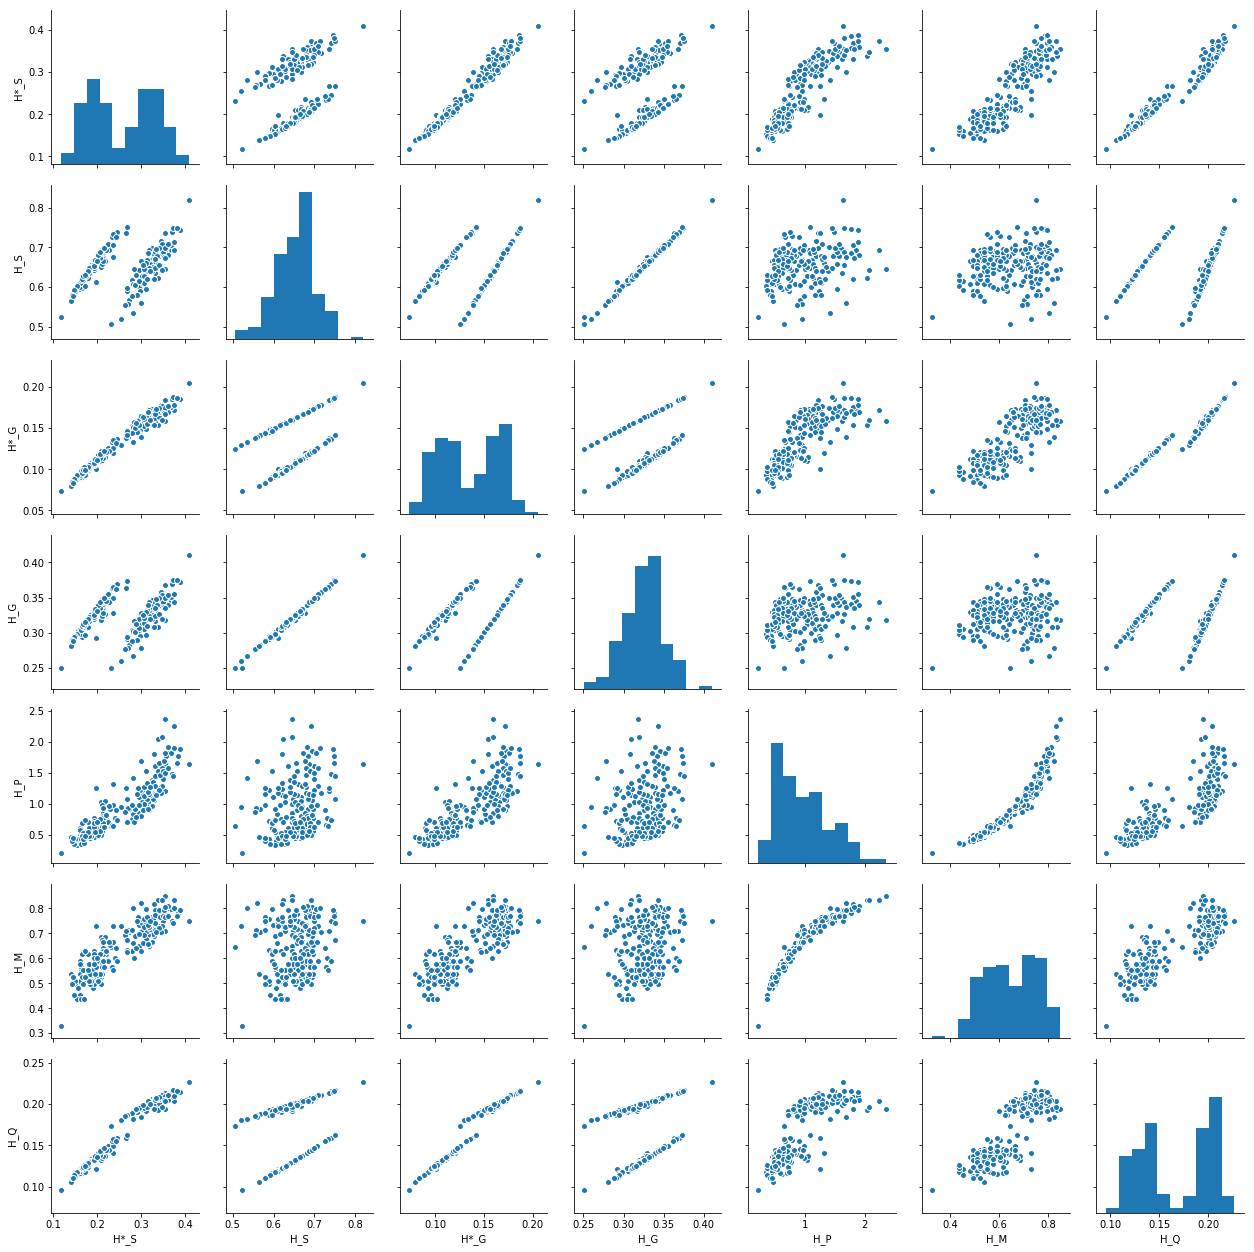
\includegraphics[width=0.6\textwidth]{images/H_2.png}
    \caption{H' en fonction de H (2 classes)}
    \label{img:H_2}
\end{figure}

\begin{figure}[H]

	\center 
	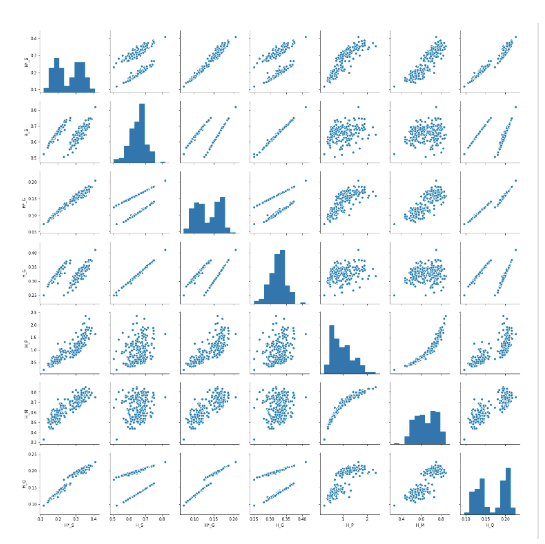
\includegraphics[width=0.6\textwidth]{images/H_3.png}
    \caption{H' en fonction de H (3 classes)}
    \label{img:H_3}
\end{figure}

\begin{figure}[H]

	\center 
	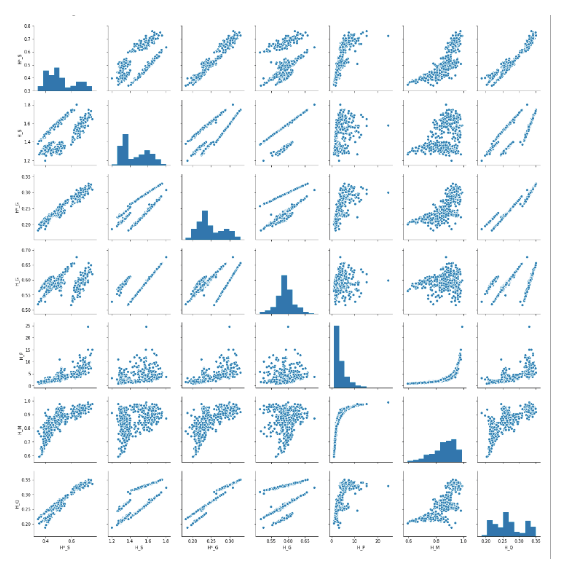
\includegraphics[width=0.6\textwidth]{images/H_5.png}
    \caption{H' en fonction de H (5 classes)}
    \label{img:H_5}
\end{figure}

Pour chaque cas, on remarque que les mesures suivantes sont corrélées
linéairement :
\begin{itemize}
    \item $H^*_S$ et $H^*_G$
    \item $H_G$ et $H_S$
\end{itemize}

Et les mesures suivantes sont corrélées quadratiquement :
\begin{itemize}
    \item $H_P$ et $H_M$
    \item $H_Q$ et $H^*_S$
\end{itemize}

\subsection{Algorithme de construction d'arbres de décision paramétré par une
mesure de discrimination}

En reprenant essentiellement RDMT, l'algorithme~\ref{alg:build-tree} est un
classifieur paramétré par une mesure de discrimination H (d'ordre ou non) et par
3 critères d'arrêt. Comme RDMT, cet algorithme ne produit pas un arbre
globalement monotone. Néanmoins, si les données sont monotone-consistentes et si
H tient compte de la relation graduelle entre les valeurs d'attributs et les
valeurs de classe, alors cette méthode garantit une forme plus faible de
monotonie (appelée \textit{rule monotonicity}). 

RDMT et notre algorithme diffèrent sur deux points :
\begin{itemize}
    \item Lorsqu'une feuille est créée, on lui assigne la classe majoritaire parmi les exemples ayant servi à sa
construction
    \item On distingue deux mesures de discrimination: l'une doit
être minimisée pour le partitionnement et l'autre permet de déterminer l'arrêt. Dans la suite, la deuxième mesure utilisée sera toujours $H_S$.
\end{itemize}

Comme l'on se restreint à des arbres de décision binaires, les données doivent
être partitionnées en deux sous-ensembles à chaque étape de l'induction. Cette
partition se fait en divisant l'ensemble courant $\Omega_{\alpha}$ selon
l'attribut $a^*$ qui respecte le plus la contrainte de monotonie, i.e. celui
dont la valeur $x^*_{j_s}$ minimise $H(\lambda|a^{x_{j_s}}_j)$, pour $j=1,...,m,
s=1,...t_j-1$. 

Etant donné une mesure de discrimination $H^*$, \textit{DISCRETIZE}
(algorithme~\ref{alg:discretize}) permet de récupérer, pour chaque $a_j \in
\mathcal{A}$, le seuil de coupure minimisant la valeur de H ainsi que cette
dernière. On parcourt tous les seuils de coupure $x_{j_s}$ de $a_j$
pour trouver $x^*_{j}$ minimisant $H(\lambda|a^{x_{j_s}}_j)$, soit :

$$ x^*_{j} = arg\,min \{H(\lambda|a^{x_{j_s}}_j), s=1,...,t_j -1\}$$

\begin{algorithm}[H]
\caption{Discrétisation}
\label{alg:discretize}
\begin{algorithmic}
\Procedure{discretize}{$H^*, \Omega$}
\State \Comment{$H^*$ : mesure de discrimination construite de façon hiérarchique}
\State \Comment{$\Omega$ : base de données étiquetées}
\State \Comment{$a_j$: attribut à discrétiser}

\State $n\gets$ $| \Omega |$ 
\State $T \gets $ matrice dont la première colonne contient les valeurs de $a_j(\omega_i)$ triées par ordre croissant, la deuxième, les valeurs de $\lambda(\omega_i)$ triées selon $a_j(\omega_i)$, et la troisième, les $i=1,...,n$ triés selon $a_j(\omega_i)$, pour tout $\omega_i \in \Omega$.
%\State $T[:,0]\gets$ les valeurs de $a_j(w_i)$ triées par ordre croisant, $\forall w_i \in \Omega$
%\State $T[:,1]\gets$ les valeurs de $\lambda(w_i)$ triées selon $T[:,0]$, $\forall w_i \in \Omega$
%\State $T[:,2]\gets$ les $w_i \in \Omega$ triés selon $T[:,0]$
\State $U\gets \{a_j(w_i) : \forall \omega_i \in \Omega\}$ \Comment{valeurs uniques de $a_j(\omega_i)$ pour tout $\omega_i \in \Omega$} \\

\State $a^{b}_j(\omega_i) \gets 1, \forall w_i \in \Omega$ \Comment{valeur de l'attribut $a_j$ binarisée i.e $a^{b}_j(\omega_i) = 0$ si $a_j(\omega_i) \leq x_{j_s}$, 1 sinon, pour $x_{j_s}$ fixé}
\State $[\omega_i]^{\leq}_{a^{b}_j} \gets \Omega, \forall w_i \in \Omega$ 
\State $[\omega_i]a_i]^{\leq}_{\lambda} \gets \{\omega_h \in \Omega : \lambda(\omega_i) \leq \lambda(\omega_h)\}$ \\

\State $S \gets \varnothing $ \Comment{seuils de coupure considérés}
\State $E \gets \varnothing $ \Comment{valeurs de $H^*$ obtenues pour chaque seuil de coupure $s \in S$}
\State V $\gets \varnothing $ \Comment{ensemble des $\omega \in \Omega$ déjà visités} \\

\For{$v \in U$}
    \State $\Omega_{v} \gets \{\omega_i \in \Omega : a_j(\omega_i) = v\}$
    \State $C_{v} \gets \{c \in C : \exists \omega_h \in \Omega_{v}, \lambda(\omega_h) = c\}$
    \State $v' \gets$ valeur suivante dans U
    \State $\Omega_{v'} \gets \{\omega_i \in \Omega : a_j(\omega_i) = v'\}$
    \State $C_{v'} \gets \{c \in C : \exists \omega_h \in \Omega_{v'}, \lambda(\omega_h) = c\}$
    \State $V \gets V \cup \{\Omega_{v}\}$    
    \State $a^{b}_j(\omega_i) \gets 0$ pour tout $\omega_i \in \Omega_{v}$ 
    \State $x_{j_s}\gets \frac{v + v'}{2}$\\
    
    \If{$C_{v'} \neq C_{v}$}
    	\State $[\omega_i]_{a^{b}_j} \gets \Omega, \forall \omega_i \in V$
        \State $\bar{V} \gets \Omega \setminus V$ \Comment{ensemble des $\omega \in \Omega$ non visités}
        \State $[\omega_i]^{\leq}_{a^{b}_j} \gets \bar{V}, \forall \omega_i \in \bar{V}$
        \State $S \gets S \cup \{x_{j_s}\}$
        \State $E \gets E \cup \{H^*(\lambda | a^{b}_j)\}$
    \EndIf
\EndFor

\State \textbf{return} $\min E, arg\,min_{s \in S} E $ \Comment{retourner la valeur d'entropie minimale et le seuil de coupure permettant de l'obtenir}
\EndProcedure
\end{algorithmic}
\end{algorithm}


\begin{algorithm}[H]
\caption{Construction de l'arbre}
\label{alg:build-tree}
\begin{algorithmic}
\Procedure{build\_dt}{$\Omega_{\alpha}$, $H^*$, H, $\epsilon$, $\Delta$, $n_{min}$, $\lambda$, $\delta$}
\State \Comment{$\Omega_{\alpha}$ : base de données étiquetées}
\State \Comment{$H^*$ : mesure de discrimination utilisée pour le
    partitionnement}
\State \Comment{$H$ : mesure de discrimination utilisée pour déterminer l'arrêt }
\State \Comment{$\epsilon$ : limite inférieure pour H}
\State \Comment{$\Delta$ : longueur maximale d'un chemin de la racine à une feuille}
\State \Comment{$n_{min}$ : taille minimale pour $\Omega_{\alpha}$}
\State \Comment{$\lambda$ : fonction d'étiquetage}
\State \Comment{$\delta$ : longueur du chemin de la racine au noeud courant}

\State $h \gets H(\Omega_{\alpha}, \lambda)$

\If{$h < \epsilon$ \OR $| \Omega_{\alpha} | < n_{min}$ \OR $\forall \omega_i,
    \omega_h \in \Omega_{\alpha}, \lambda(\omega_i) = \lambda(\omega_h)$ \OR $\delta > \Delta$}
    \State $c_{\alpha} \gets c$ tel que $|\{\omega_i \in \Omega_{\alpha}:
        \lambda(\omega_i) = c\}| \geq |\{\omega_i \in \Omega_{\alpha}:
        \lambda(\omega_i) \neq c\}|$
    \State \textbf{return} LEAF($c_{\alpha}, \Omega$) \\
    %\State \textbf{return} $\{c\}$ tel que $|\{\omega_i \in \Omega_{\alpha}:
    %\lambda(\omega_i) = c\}| \geq |\{\omega_i \in \Omega_{\alpha}:
    %\lambda(\omega_i) \neq c\}|$ \\ 
\EndIf

\State $m\gets$ nombre d'attributs dans $\Omega$
\State $S\gets \varnothing $ \Comment{pour chaque $a_j \in \mathcal{A}$,
    contient $x_{j_{*}}= arg\,min \{H(\lambda | a^{x_{j_s}}_j), s=1,...,t_{j} - 1$\}}
\State $E\gets \varnothing $ \Comment{pour chaque $a_j \in \mathcal{A}$,
    contient $min \{H(\lambda | a^{x_{j_s}}_j), s=1,...,t_j - 1\}$}\\

\For{$a_j$=0 to m-1}
    \If{$a_j(\omega_i) = a_j(\omega_h), \forall \omega_i, \omega_h \in
    \Omega_{\alpha}$} \State $S \gets S \cup \{\infty\}$
    	\State $E \gets E \cup \{\infty\}$
    \Else
        \State $x_{j_*}, h \gets$ DISCRETIZE($H^*, \Omega_{\alpha}, a_j$) 
        \State $S \gets S \cup \{x_{j_*}\}$
        \State $E \gets E \cup \{h\}$ \\
    \EndIf
\EndFor

\State $x_* \gets arg\,min_{s \in S} E$ %seuils[argmin(entropies)]
\State $a^{x_*}_*\gets arg\,min_{a_j \in \mathcal{A}} E $ \\ %argmin(entropies)

\State $\Omega_{\leq}, \Omega_{\geq}\gets$ DIVIDE($\Omega_{\alpha}, a^{x_*}_*,
    x_*$) 

\If{$| \Omega_{\leq} | = 0$}
    \State \textbf{return} $\{c\}$ tel que $|\{\omega_i \in \Omega_{\geq}:
    \lambda(\omega_i) = c\}| \geq |\{\omega_i \in \Omega_{\geq}:
    \lambda(\omega_i) \neq c\}|$
\EndIf

\If{$| \Omega_{\geq} | = 0$}
    \State \textbf{return} $\{c\}$ tel que $|\{\omega_i \in \Omega_{\leq}
    \lambda(\omega_i) = c\}| \geq |\{\omega_i \in \Omega_{\leq}:
    \lambda(\omega_i) \neq c\}|$
\EndIf

\State $\mathcal{T}_{\leq}\gets$ BUILD\_DT($\Omega_{\leq}, H^*, H, \epsilon, \Delta,
    n_{min}, \lambda, \delta +1$) 
\State $\Gamma_{\geq}\gets$
    BUILD\_DT($\mathcal{T}_{\geq}, H^*, H, \epsilon, \Delta, n_{min}, \lambda, \delta
    +1$)
\State $\mathcal{T} \gets$ TREE($\{a^{x_*}_*\}, \mathcal{T}_{\leq}, \mathcal{T}_{\geq}$)
\State \textbf{return} $\mathcal{T}$

\EndProcedure
\end{algorithmic}
\end{algorithm}

%Le critère de partitionnement \textit{DISCRETIZE} est donné par l'algorithme~\ref{alg:discretize}.
%Pour un attribut $a_j$, il consiste à parcourir tous les seuils de coupure
%$x_{j_s}$ de $a_j$ pour trouver $x$ minimisant $H(\lambda|a^{x_{j_s}}_j)$, soit :
%
%$$ x = arg\,min \{H(\lambda|a^{x_{j_s}}_j), s=1,...,t_j -1\}$$
%
%\begin{algorithm}[H]
%\caption{Discrétisation}
%\label{alg:discretize}
%\begin{algorithmic}
%\Procedure{discretize}{$H^*, \Omega$}
%\State \Comment{$H^*$ : mesure de discrimination construite de façon hiérarchique}
%\State \Comment{$\Omega$ : base de données étiquetées}
%\State \Comment{$a_j$: attribut à discrétiser}
%
%\State $n\gets$ $| \Omega |$ 
%\State $T \gets $ matrice dont la première colonne contient les valeurs de $a_j(\omega_i)$ triées par ordre croissant, la deuxième, les valeurs de $\lambda(\omega_i)$ triées selon $a_j(\omega_i)$, et la troisième, les $i=1,...,n$ triés selon $a_j(\omega_i)$, pour tout $\omega_i \in \Omega$.
%%\State $T[:,0]\gets$ les valeurs de $a_j(w_i)$ triées par ordre croisant, $\forall w_i \in \Omega$
%%\State $T[:,1]\gets$ les valeurs de $\lambda(w_i)$ triées selon $T[:,0]$, $\forall w_i \in \Omega$
%%\State $T[:,2]\gets$ les $w_i \in \Omega$ triés selon $T[:,0]$
%\State $U\gets \{a_j(w_i) : \forall \omega_i \in \Omega\}$ \Comment{valeurs uniques de $a_j(\omega_i)$ pour tout $\omega_i \in \Omega$} \\
%
%\State $a^{b}_j(\omega_i) \gets 1, \forall w_i \in \Omega$ \Comment{valeur de l'attribut $a_j$ binarisée i.e $a^{b}_j(\omega_i) = 0$ si $a_j(\omega_i) \leq x_{j_s}$, 1 sinon, pour $x_{j_s}$ fixé}
%\State $[\omega_i]^{\leq}_{a^{b}_j} \gets \Omega, \forall w_i \in \Omega$ 
%\State $[\omega_i]a_i]^{\leq}_{\lambda} \gets \{\omega_h \in \Omega : \lambda(\omega_i) \leq \lambda(\omega_h)\}$ \\
%
%\State $S \gets \varnothing $ \Comment{seuils de coupure considérés}
%\State $E \gets \varnothing $ \Comment{valeurs de $H^*$ obtenues pour chaque seuil de coupure $s \in S$}
%\State V $\gets \varnothing $ \Comment{ensemble des $\omega \in \Omega$ déjà visités} \\
%
%\For{$v \in U$}
%    \State $\Omega_{v} \gets \{\omega_i \in \Omega : a_j(\omega_i) = v\}$
%    \State $C_{v} \gets \{c \in C : \exists \omega_h \in \Omega_{v}, \lambda(\omega_h) = c\}$
%    \State $v' \gets$ valeur suivante dans U
%    \State $\Omega_{v'} \gets \{\omega_i \in \Omega : a_j(\omega_i) = v'\}$
%    \State $C_{v'} \gets \{c \in C : \exists \omega_h \in \Omega_{v'}, \lambda(\omega_h) = c\}$
%    \State $V \gets V \cup \{\Omega_{v}\}$    
%    \State $a^{b}_j(\omega_i) \gets 0$ pour tout $\omega_i \in \Omega_{v}$ 
%    \State $x_{j_s}\gets \frac{v + v'}{2}$\\
%    
%    \If{$C_{v'} \neq C_{v}$}
%    	\State $[\omega_i]_{a^{b}_j} \gets \Omega, \forall \omega_i \in V$
%        \State $\bar{V} \gets \Omega \setminus V$ \Comment{ensemble des $\omega \in \Omega$ non visités}
%        \State $[\omega_i]^{\leq}_{a^{b}_j} \gets \bar{V}, \forall \omega_i \in \bar{V}$
%        \State $S \gets S \cup \{x_{j_s}\}$
%        \State $E \gets E \cup \{H^*(\lambda | a^{b}_j)\}$
%    \EndIf
%\EndFor
%
%\State \textbf{return} $\min E, arg\,min_{s \in S} E $ \Comment{retourner la valeur d'entropie minimale et le seuil de coupure permettant de l'obtenir}
%\EndProcedure
%\end{algorithmic}
%\end{algorithm}

Considérons la base de la figure \ref{img:artificial-dataset} contenant 60
points à deux dimensions x et y et à 3 classes. x est l'attribut dont les valeurs sont
monotones par rapport aux valeurs de la classe. Chaque classe est représentée
par le même nombre de points. La classe 1 est
représentée par les points bleus, la 2 par les points oranges, et la 3 par les
points verts. 

\begin{figure}[H]
	\center 
	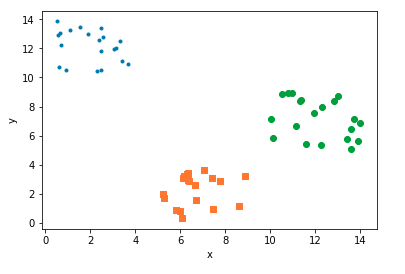
\includegraphics[width=0.6\textwidth]{images/artificial-dataset.png}
    \caption{Base de données jouet}
    \label{img:artificial-dataset}
\end{figure}

\begin{figure}[H]
	\center 
	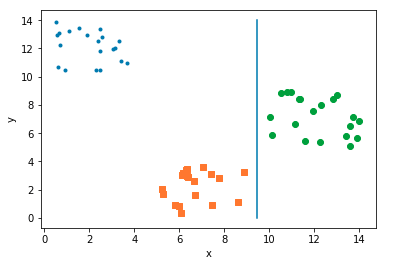
\includegraphics[width=0.6\textwidth]{images/threshold_rsdm.png}
    $$H^*_S(\lambda | \mathbf{x}) =  0.19 \leq H^*_S(\lambda | \mathbf{y}) =  0.53$$
    \caption{Seuil de coupure généré par $H^*_S$}
    \label{img:threshold_rsdm}
\end{figure}

\begin{figure}[H]
	\center 
	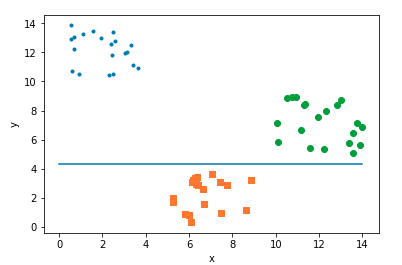
\includegraphics[width=0.6\textwidth]{images/threshold_sdm.png}
    $$H_S(\lambda | \mathbf{x}) = H_S(\lambda | \mathbf{y}) =  0.67$$
    \caption{Seuil de coupure généré par $H_S$}
    \label{img:threshold_sdm}
\end{figure}

On observe sur les figures \ref{img:threshold_rsdm} et \ref{img:threshold_sdm}
les seuils de coupures générés respectivement par $H^*_S$ et $H_S$ sur cette
base jouet. On remarque que $H^*_S$ tient compte de la monotonie des valeurs de
la classe par rapport aux valeurs de l'attribut x : la valeur d'entropie
minimale calculée pour l'attribut x est inférieure à celle calculée pour
l'attribut y. Ce n'est cependant pas le cas pour $H_S$ qui est insensible à la
monotonie : la coupure optimale sur l'axe x génère la même valeur d'entropie que
celle faite sur l'axe y.


\printbibliography
\end{document}
